%&pdflatex
\section{Avvio di Debian}\label{sec:starting-debian}
Prima di partire, raccomandiamo di collegare il computer al proprio \textit{router} di casa tramite un \textbf{cavo Ethernet} per tutto il tempo dell'installazione. Questo consentirà a Debian di configurare automaticamente le impostazioni di rete. Se invece usassimo il \textit{WiFi}, dovremmo poi configurare manualmente la rete. In questo testo, non verrà trattata la configurazione manuale della rete.

Per avviare Debian dobbiamo inserire il CD/DVD o il pendrive USB che abbiamo scritto ed entrare nel pannello di configurazione del firmware (come abbiamo fatto nel paragrafo precedente) e modificare l'ordine di priorità del boot. Infatti il firmware andrà a cercare il bootloader all'interno del nostro disco fisso --- adesso però vogliamo che lo vada a cercare all'interno del CD/pendrive.

Anche per questo non esiste una procedura standard: è necessario cercare all'interno del pannello qualcosa di simile a quanto mostrato in Figura \vref{fig:ovmf-boot-order}.

\begin{figure}[ht]
	\centering
	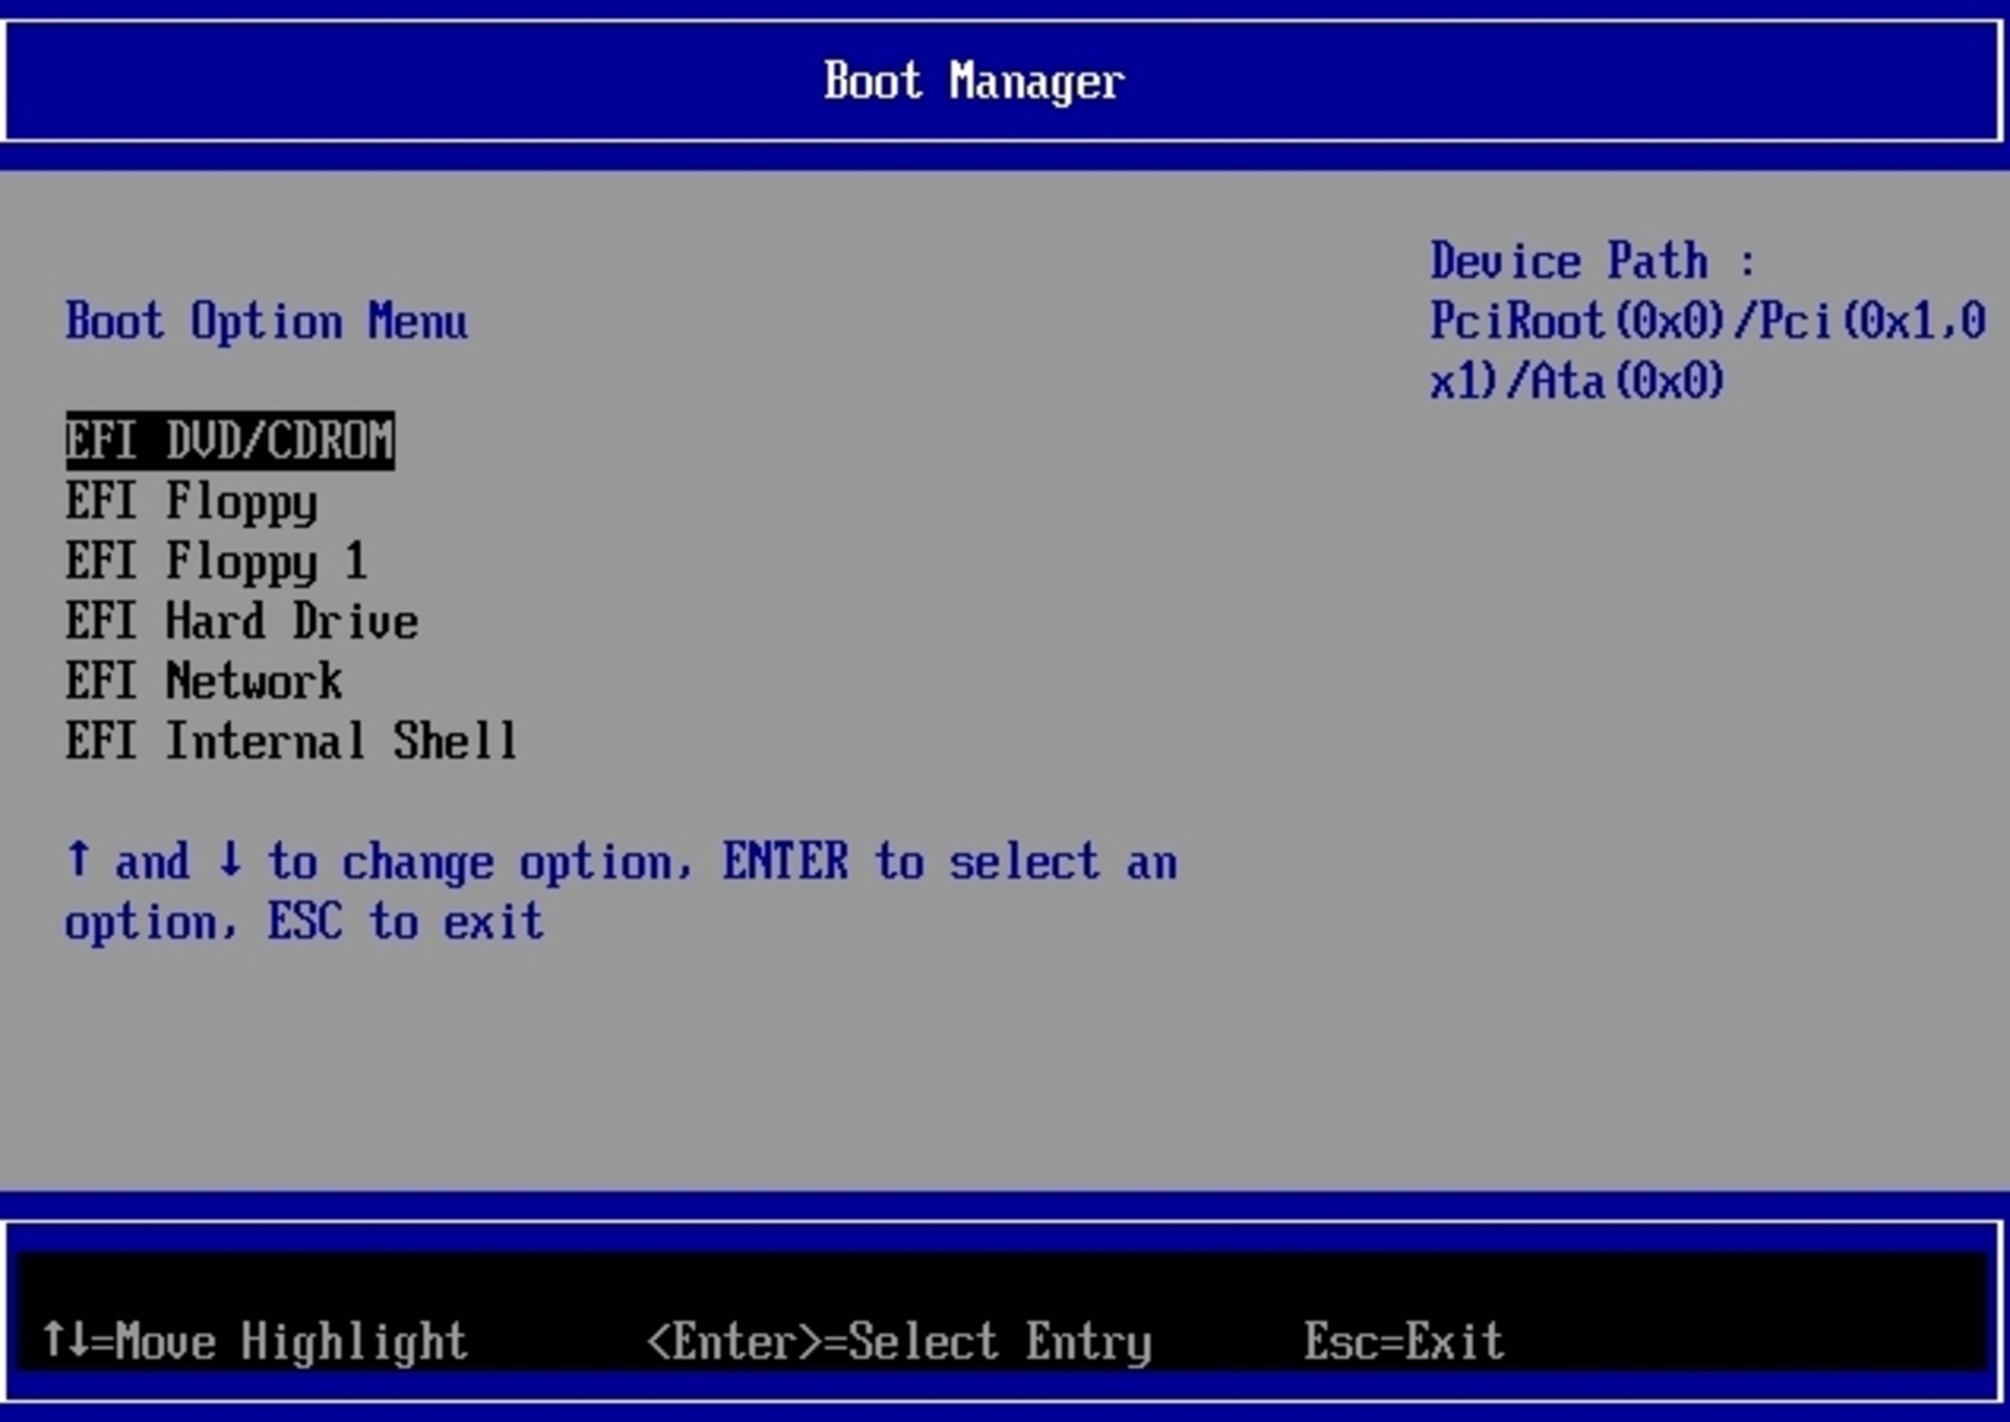
\includegraphics[resolution=600]{ovmf-boot-order}
	\caption{Ordine di boot all'interno di un pannello di configurazione di un firmware UEFI (OVMF)}
	\label{fig:ovmf-boot-order}
\end{figure}

Come è possibile vedere dall'immagine, il CD/DVD è stato messo in cima alla lista dell'ordine di avvio.

Una volta impostato correttamente l'ordine di avvio ci si ricordi di salvare la nuova configurazione. A questo punto, se tutto va bene, si avvierà Debian. Se ciò non succede, si consiglia di rivedere questo paragrafo e il precedente e di accertarsi di aver fatto tutto correttamente. La prima interfaccia che ci verrà mostrata è quella di Figura \vref{fig:debian-bootloader}.

\begin{figure}[ht]
	\centering
	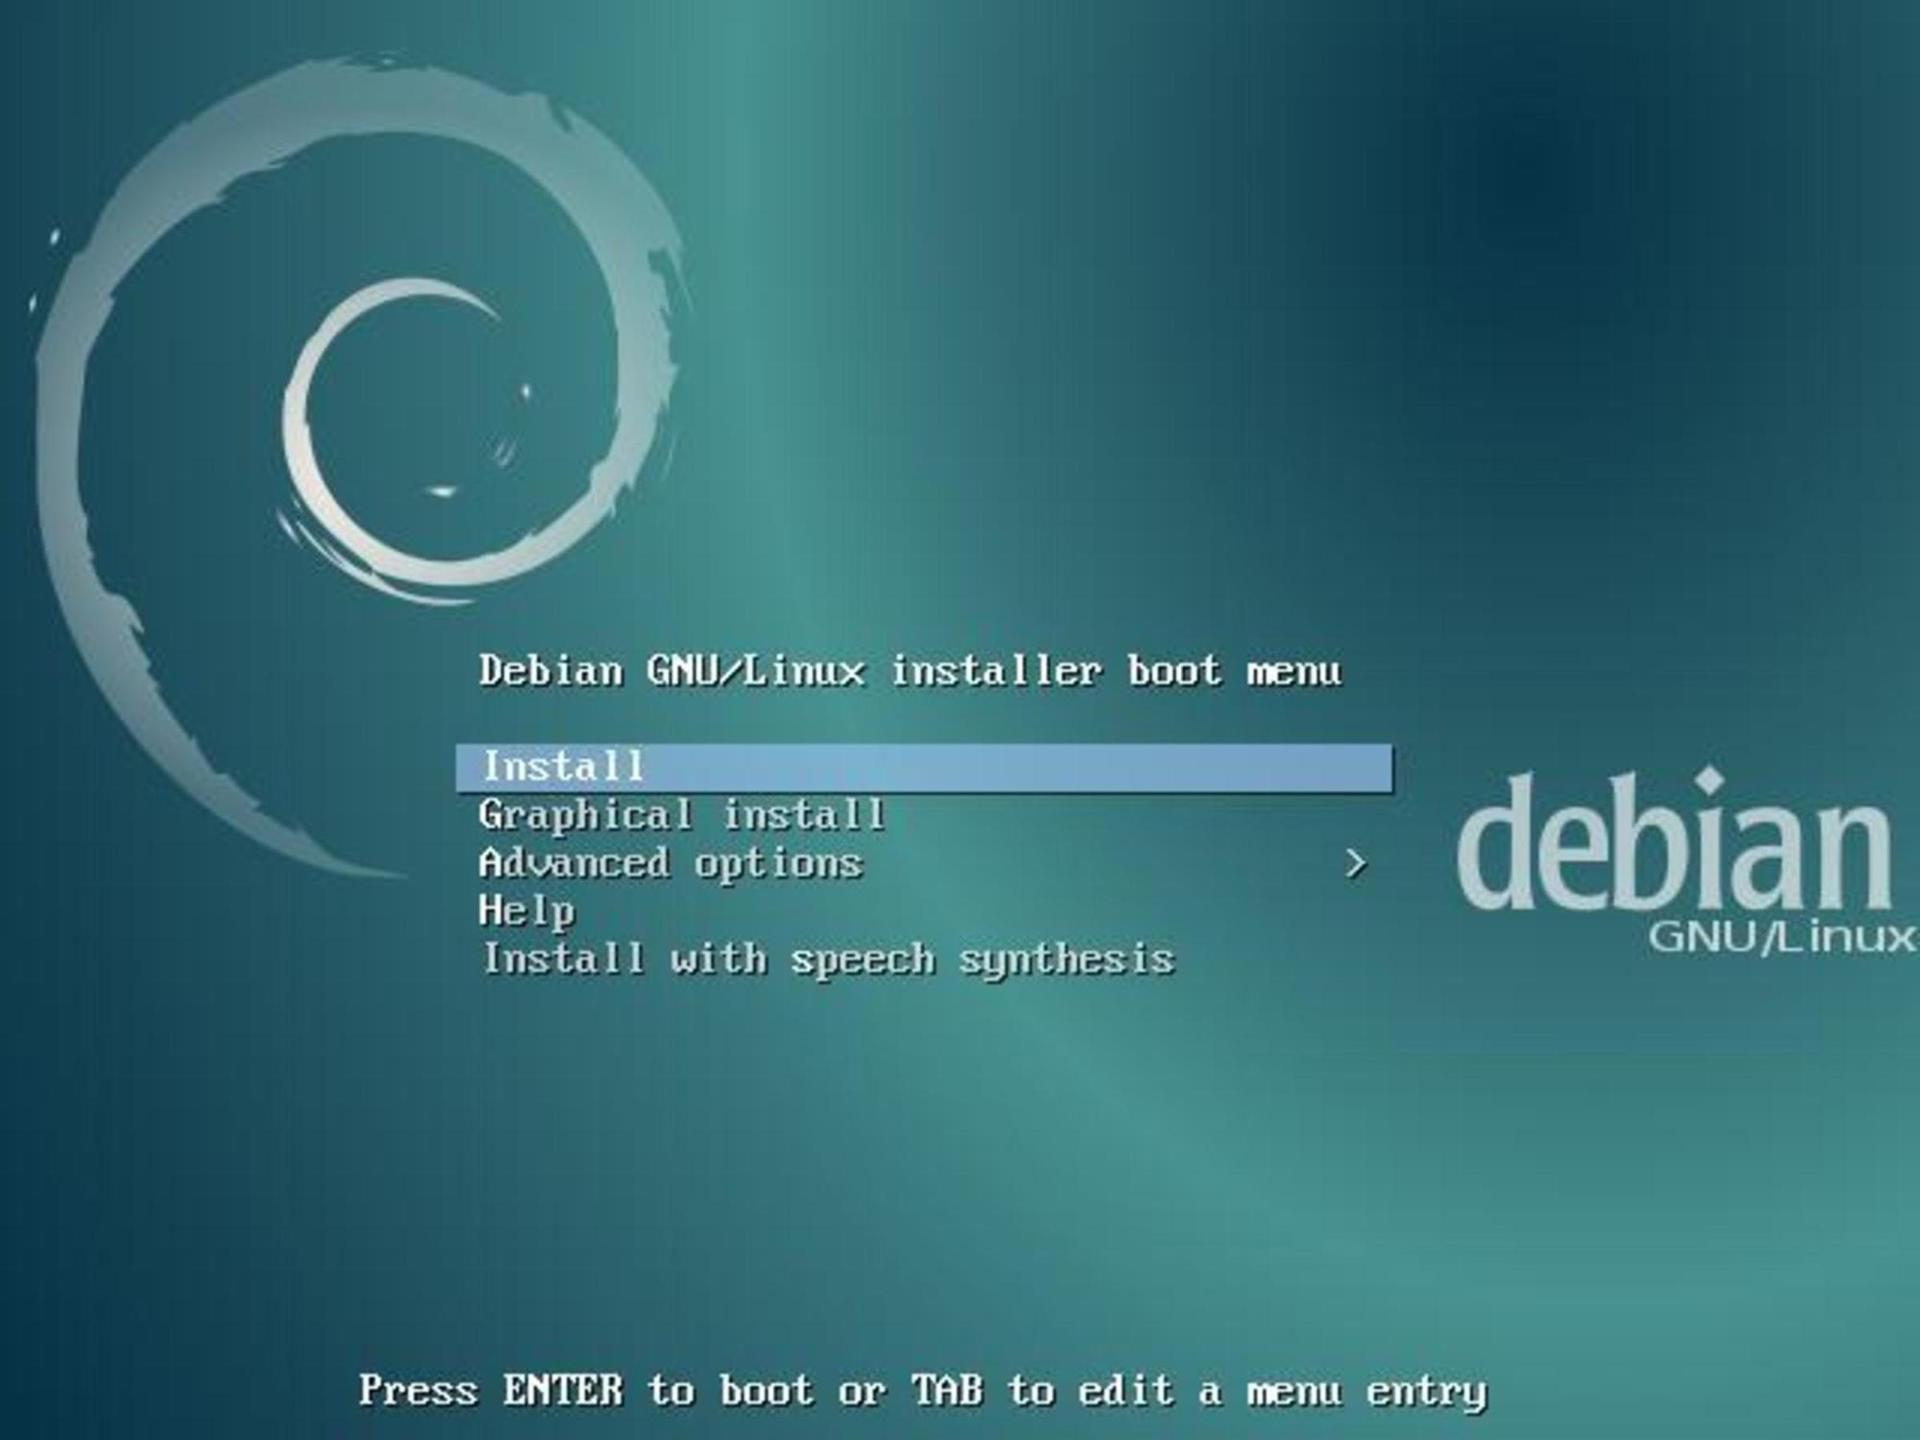
\includegraphics[resolution=600]{debian-bootloader}
	\caption{Bootloader dell'installer di Debian}
	\label{fig:debian-bootloader}
\end{figure}

Qui possiamo scegliere varie voci: la prima (\texttt{Install}) è per iniziare un'installazione da linea di comando (per utenti esperti). La terza (\texttt{Advanced options}) permette di accedere a un nuovo menu con opzioni avanzate. Le ultime due (\texttt{Help} e \texttt{Install with speech synthesis}) servono ad accedere al manuale di supporto o per avviare un'installazione vocale per ipovedenti. La seconda infine (\texttt{Graphical install}) permette di avviare un'installazione grafica.

Scegliamo con le frecce proprio la seconda voce (\texttt{Graphical install}) e premiamo invio. Partirà l'installer di Debian.
